\chapter{ANEXO}\label{chap:anexo}
\section{Instalación Labelme}\label{sec:instalacionlabelme}
La instalación de \textit{labelme}, se realizo bajo un sistema operativo Ubuntu-Linux Mint v18.0; se debe instalar las siguiente dependencias:
\begin{itemize}
\item \href{https://www.scipy.org/}{Scipy}
\item \href{http://www.numpy.org/}{Numpy}
\item \href{http://scikit-image.org/}{scikit-image}
\item \href{https://riverbankcomputing.com/software/pyqt/intro}{PyQt}
\item \href{http://matplotlib.org/}{Matplot}
\end{itemize}

Luego desde la terminal de Linux ingresamos los siguientes comandos:

\textbf{(user):sudo apt-get install labelme}

Para iniciar \textit{labelme} se ingresa desde la terminal el siguiente comando:

\textbf{(user): labelme (path/nameimage.tiff)}

\begin{figure}[H]
 \centering
  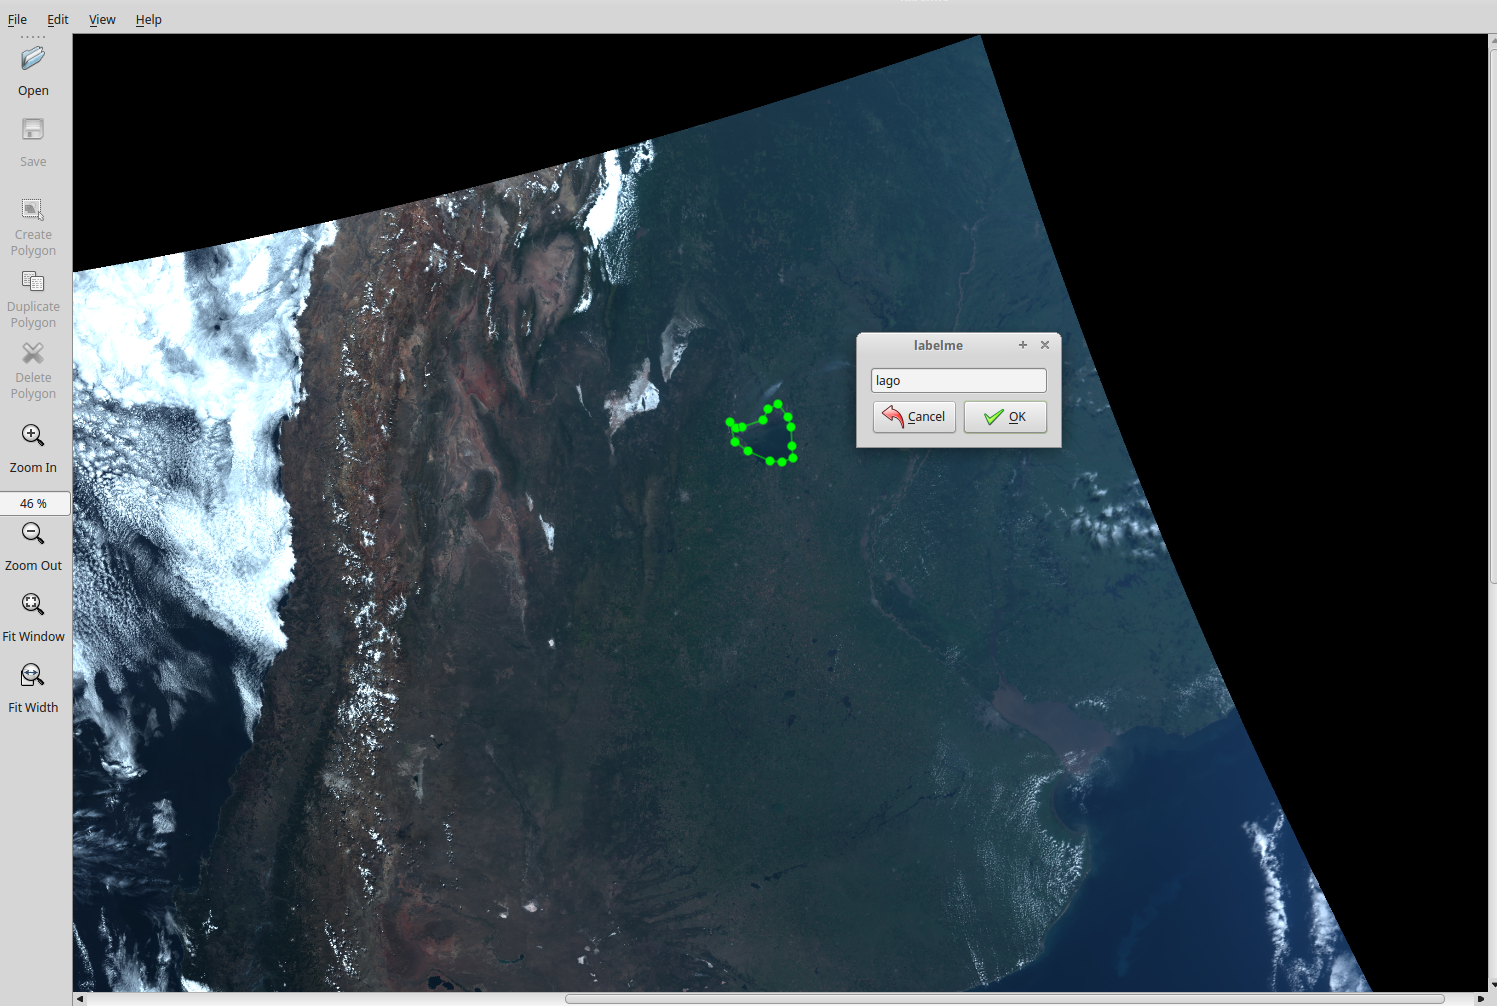
\includegraphics[height=8cm,keepaspectratio=true,clip=true]{imagenes/Apendice/labelme1.png}
  \caption{Pantalla Principal \textit{labelme}}
	\label{Fig: labelme}
\end{figure}

Las anotaciones realizas en este software se almacenará en formato JSON.

%%%%%%%%%%%%%%%%%%%%%%%%%%%%%%%%
\section{Instalación Keras}\label{sec:instalacionkeras}
Keras es una librería para hacer Deep Learning, keras esta escrita en python ejecuntandose sobre una capa superior de TensorFlow. A continuación vamos a desarrollar el proceso de instalación:

Dependencias de Keras:
\begin{itemize}
\item numpy scipy
\item scikit-learn
\item pillow
\item h5py
\end{itemize}
Luego de la instalación de las dependencias hacemos:

 \textbf{\$ sudo pip install keras}
%%%%%%%%%%%%%%%%%%%%%%%%%%%%%%%%
\section{Instalación OpenCV}\label{sec:instalacionopencv}
La instalación de OpenCV se realizo por medio del Repositorio de Ubuntu:

\$\textbf{ sudo pip install opencv-python}

La versión utilizada de OpenCV fue la 2.4.9.1 bajo Ubuntu 14.04. Para verificar la su instalación realizamos los siguiente:\\
\$ python\\
\$ import cv2\\
\$ cv2.\_version\_


%%%%%%%%%%%%%%%%%%%%%%%%%%%%%%%%
\section{Instalación Edge Proposal }\label{sec:instalacionedge}
El método para la obtención de regiones propuesta se ejecuto bajo el lenguaje MATLAB bajo la version R2013b. Se descargo el toolbox desde el repositorio \url{https://github.com/pdollar/toolbox}, se coloca en una carpeta y desde MATLAB en la pestaña Home>SetPath se agrega la correspondiente carpeta. Luego usamos la opción \textit{move to bottom} para soobrescribir las funciones predefinidas de MATLAB.

A continuación descargamos la siguiente dirección \url{https://github.com/pdollar/edges}, realizando el mismo procedimiento anterior.

%%%%%%%%%%%%%%%%%%%%%%%%%%%%%%%%%

\section{Instalación de BING}
Para la realización de BING, regiones propuestas, se realizo lo siguiente:

Clonamos el siguiente repositorio usando la herramienta GIT\\
\$\textbf{ git clone https://github.com/alessandroferrari/BING-Objectness}
Ingresamos a la carpeta Clonada y realizamos \\
\$ \textbf{make} \\
Agregamos al PYTHONPATH la siguiente dirección:\\
\$ \textbf{export PYTHONPATH=/home/..../BING-Objectness/build} \\

Para La ejecución de una sola imagen cambiamos los parámetros del archivo JSON bing\_params.json \\
Ejecutamos luego el archivo pasando una imagen\\
\$ \textbf{python bing.py /home/...../BING-Objectness/doc/bing\_params.json /home/...../bender.jpeg}

%%%%%%%%%%%%%%%%%%%%%%%%%%
\section{Descargas y Recolección de Imágenes}
Se descargaron las imágenes del sitio de la pagina oficial de \ac{conae} \url{http://www.conae.gov.ar/index.php/espanol/}, para la obtención de las imágenes nos dirigimos a
la solapa \textit{Catálogo de imágenes y productos}:

\begin{figure}[H]
 \centering
  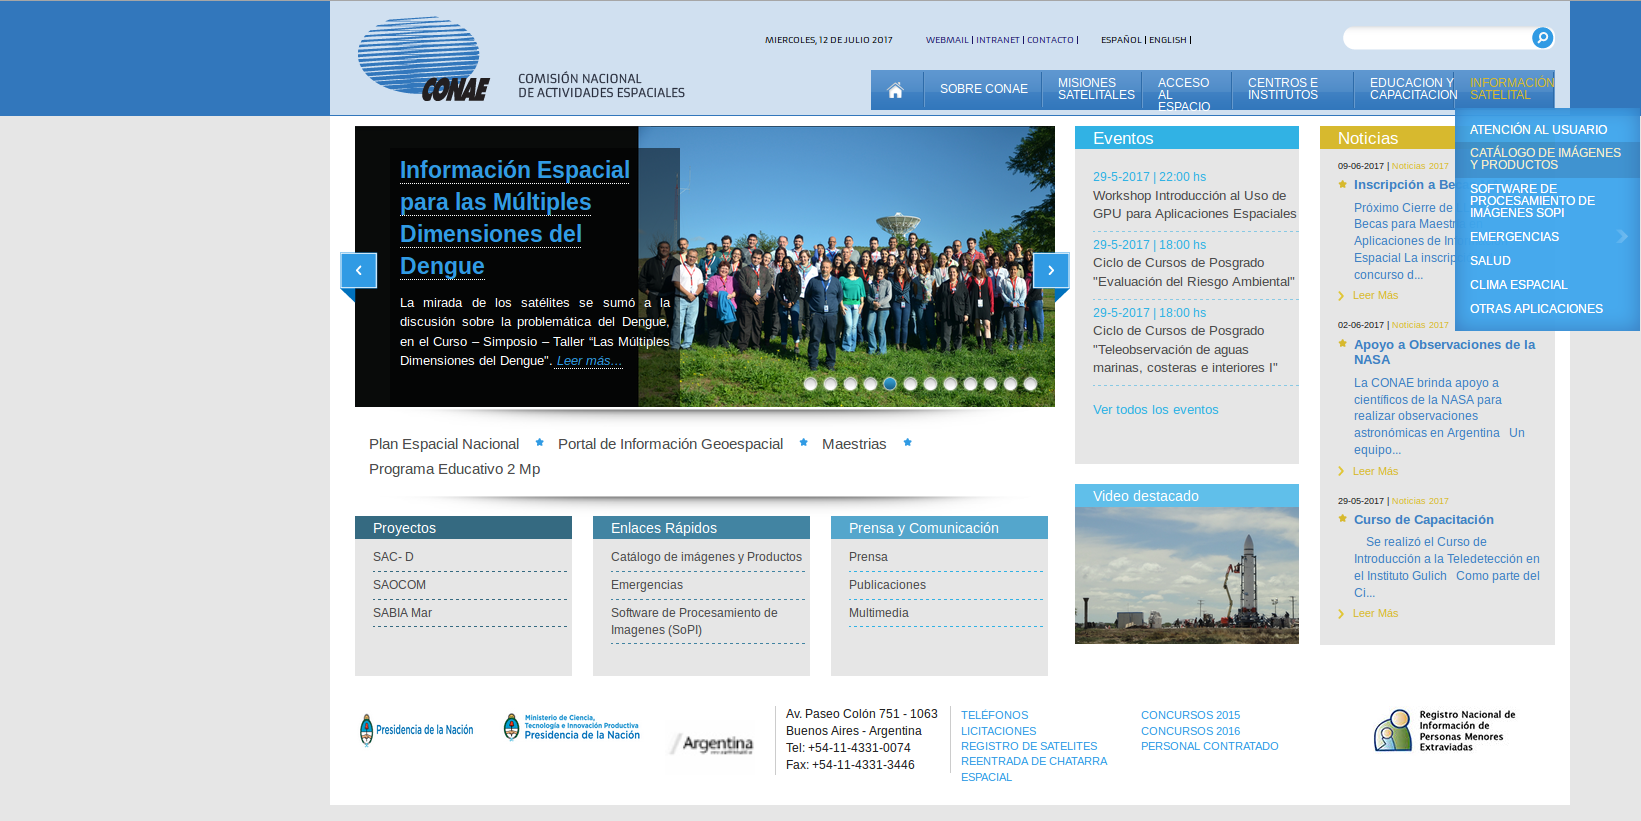
\includegraphics[height=8cm,keepaspectratio=true,clip=true]{imagenes/Apendice/conaepag.png}
  \caption{Pantalla Principal CONAE}
\end{figure}
Luego en las secciones de la izquierda de la pagina seleccionamos Aqua, Terra correspondiente al sensor modis o NPP para viirs.
\begin{figure}[h]
 \centering
  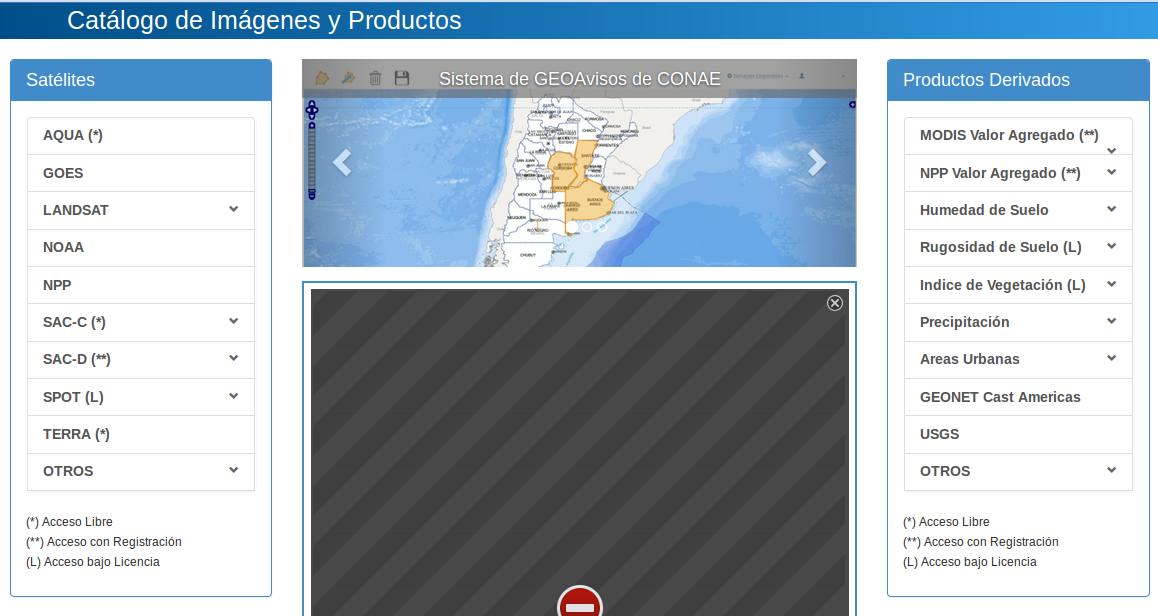
\includegraphics[height=8cm,keepaspectratio=true,clip=true]{imagenes/Apendice/conaepag1.png}
  \caption{Pantalla Principal CONAE}
\end{figure}
Para la descargas de las imágenes se debe autenticar, si no posee un usuario debe darse de alta en el sistema. Una vez autenticado podemos buscar por fecha, región, latitud,
longitud o nombre de la imagen.
\begin{figure}[h]
 \centering
  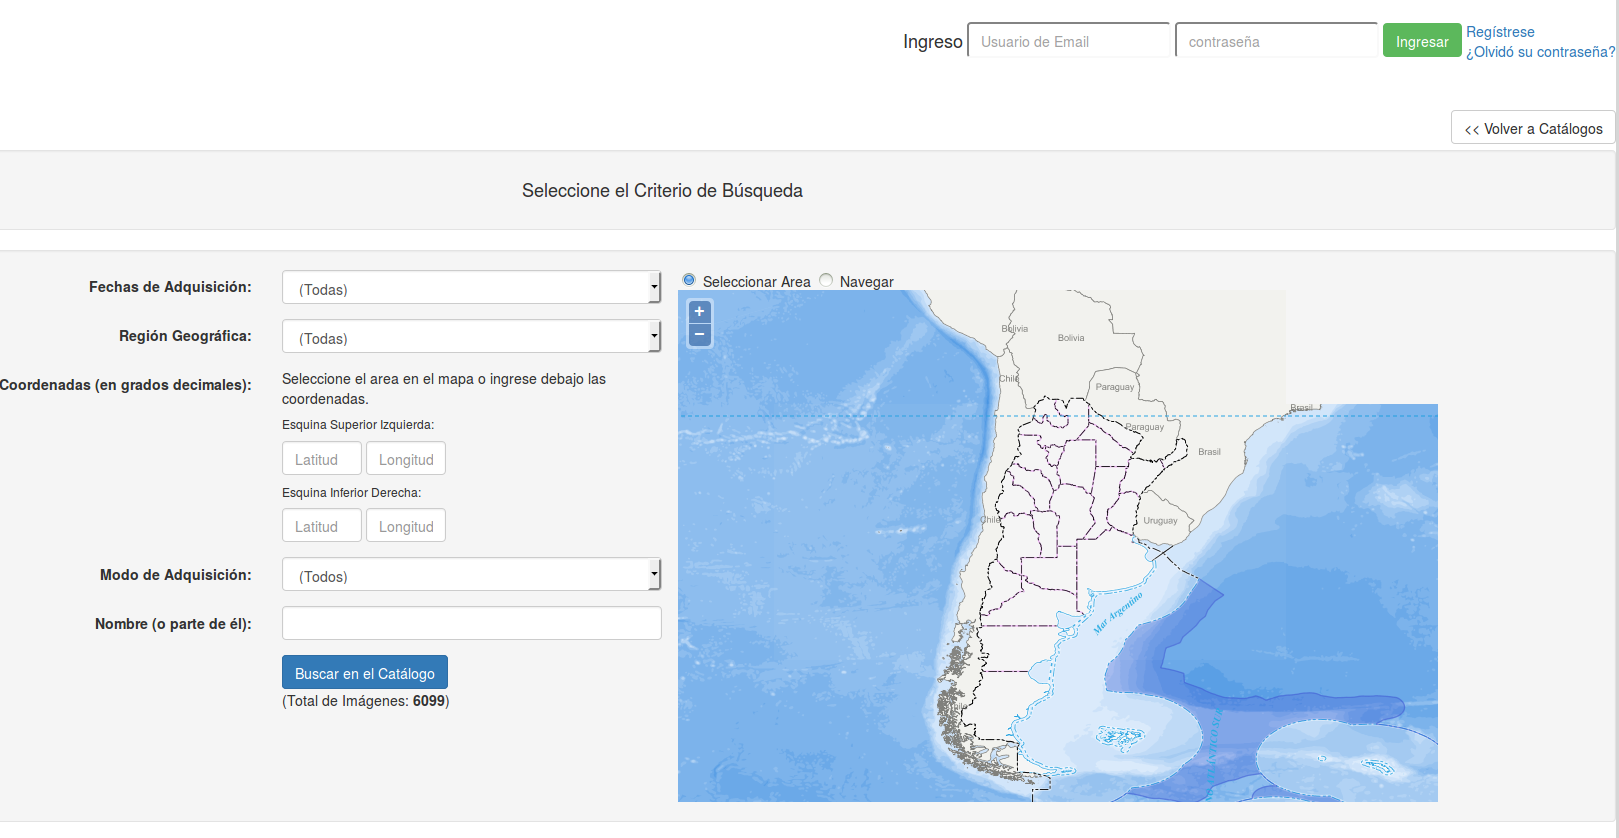
\includegraphics[height=8cm,keepaspectratio=true,clip=true]{imagenes/Apendice/conaepag2.png}
  \caption{Autenticación de usuario}
\end{figure}
Una vez seleccionada la imagen a descargar nos aparece las características de la imagen junto con las bandas que deseamos y su correspondiente archivo de georeferenciación.
\begin{figure}[H]
 \centering
  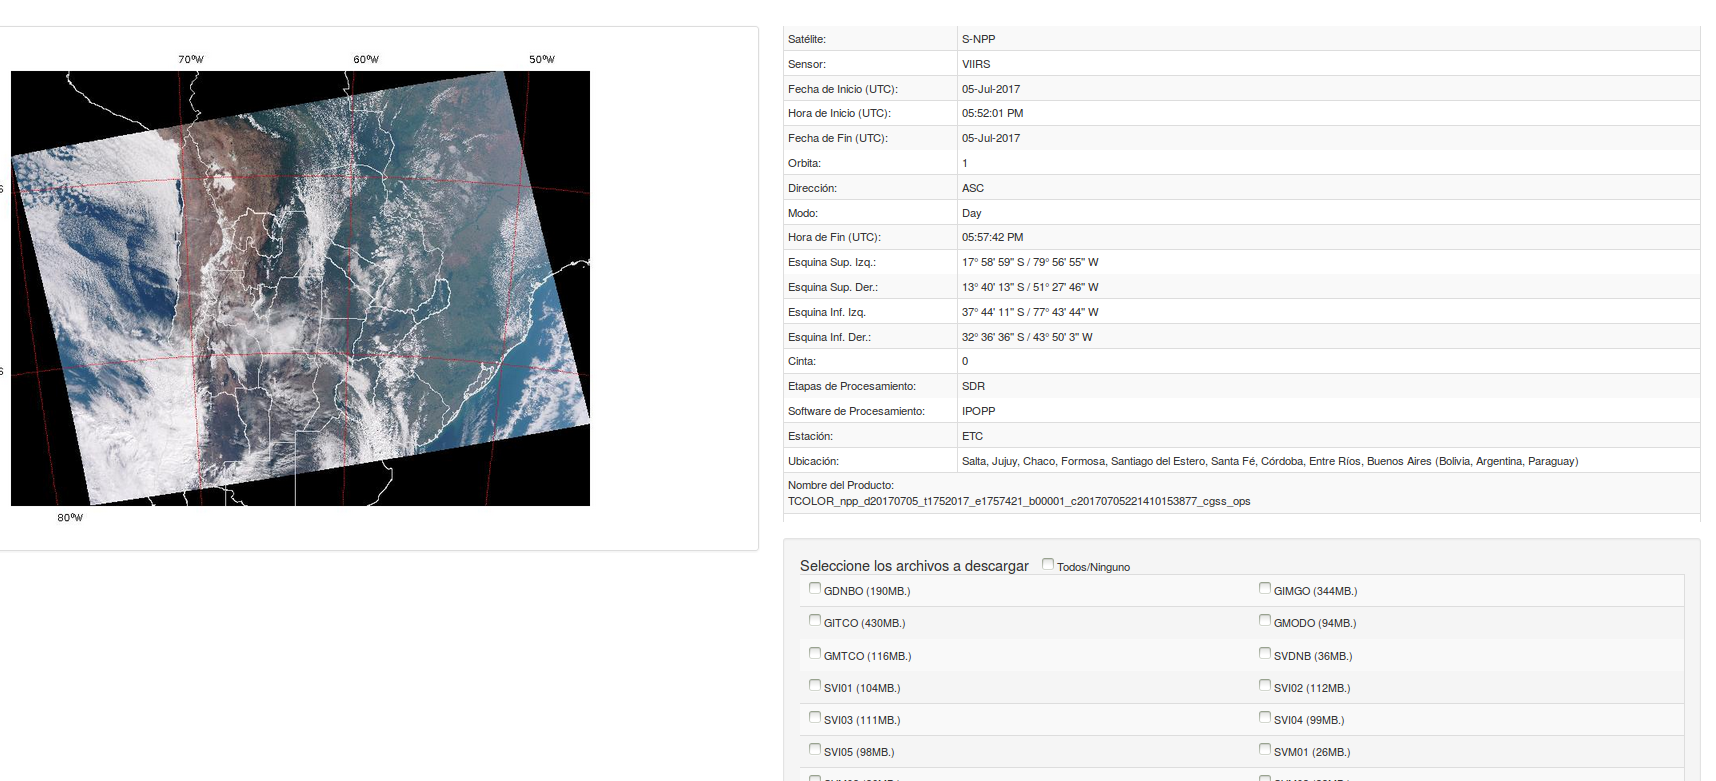
\includegraphics[height=8cm,keepaspectratio=true,clip=true]{imagenes/Apendice/conaepag3.png}
  \caption{Descarga de Imagen}
\end{figure}
%%%%%%%%%%%%%%%%%%%%%%%%%%%%%%%%%%%%%%%%%%%%%%%%%

\subsection{Recolección de Imágenes}\label{sub:recolecciondeimagen}

En esta sección vamos a desarrollar los pasos que se siguieron para la obtención de las imágenes; para esto dividiremos en dos partes las tareas realizadas por un lado se realizo la descargas de las imágenes y por otro el pre-procesamiento de las mismas. El primer paso hacemos  referencia a la descarga manual de los datos conseguidos a través de la pagina oficial de \ac{conae}; el segundo punto al que llamamos pre-procesamiento se realizaron las conversiones de los datos como se menciona en la seccion anterior \ref{sec:datosutilizados}. Para poder llevar a cabo esta ultima tarea se utilizo la herramienta de procesamiento de imágenes ENVI \ref{sub:enviSoft}, software para el análisis de imágenes. Este software nos proporciona diferentes herramientas para la manipulación y procesamiento  de  una imagen satelital, de las cuales podemos mencionar la \textit{VIIRS Conversion Toolkit}, herramienta nos permite trabajar con imágenes del instrumento \ac{viirs}, pudiendo aplicar a las imágenes correcciones geométricas, geo-referenciacion y re-proyecciones entre las diferentes funcionalidades que nos brinda. 

En este proceso de conversión de imágenes se realizaron diversos pasos para la obtención de las imágenes finales de los cuales se detallan a continuación:

\begin{enumerate}

\item Inicio, pantalla principal ENVI:
	\begin{figure}[H]\centering
		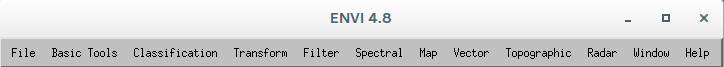
\includegraphics[height=1.5cm,keepaspectratio=true,clip=true]{imagenes/recoleccion/envi1.png}
  		\caption{Pantalla Principal ENVI} \label{Fig: envi1}
	\end{figure}


\item Procesamiento: abrir la herramienta \textit{VIIRS Conversion Toolkit} e ingresar los archivos de cada banda adjuntando el archivo  geo-referenciado, para realizar la carga de la imagen manual(figura: \ref{Fig: envi2}).

\begin{figure}[H] \centering
  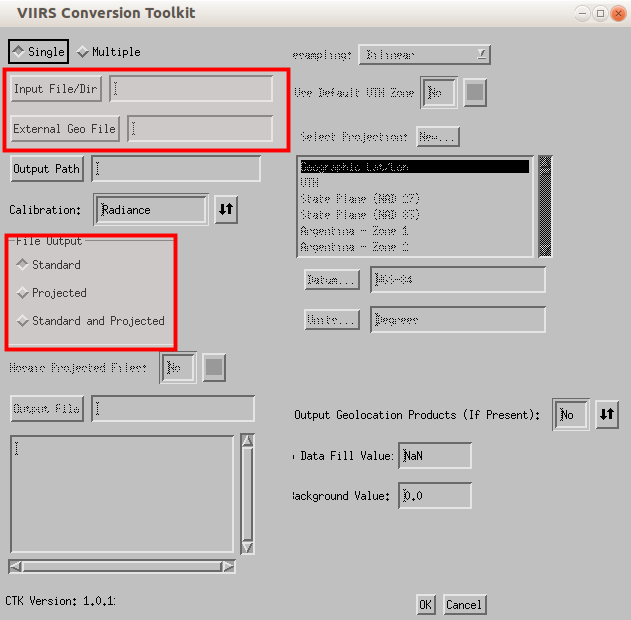
\includegraphics[height=9cm,keepaspectratio=true,clip=true]{imagenes/recoleccion/envi2.png}
  \caption{Cargar Bandas ENVI Toolkit} \label{Fig: envi2}
\end{figure}

\item Re-proyección de imagen: adjuntar bandas a utilizar; se debe asignar de acuerdo al color que corresponda cada banda (RGB) (figura: \ref{Fig: envi3}).
 
\begin{figure}[H]
 \centering
  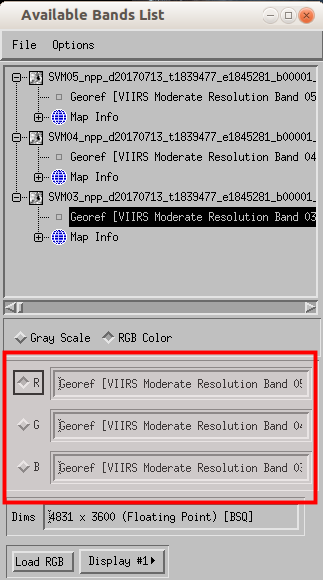
\includegraphics[height=9cm,keepaspectratio=true,clip=true]{imagenes/recoleccion/envi3.png}
  \caption{Ejemplo re-proyección \textit{True Color}}
	\label{Fig: envi3}
\end{figure}

\end{enumerate}

La imagen resultante luego de esta serie de pasos  son las que se puede ver en la figura \ref{Fig: bandas543}.

%%%%%%%%%%%%%%%%%%%%%%%%%%
\section{Instalación de Eclipse}\label{sec:instalacionEclipse}
Para la instalación del ID Eclipse se debe seguir los siguientes pasos:

Debemos ingresar a la siguiente url: http://www.eclipse.org/downloads/ y pulsar Downloads.
\begin{figure}[H]
 \centering
  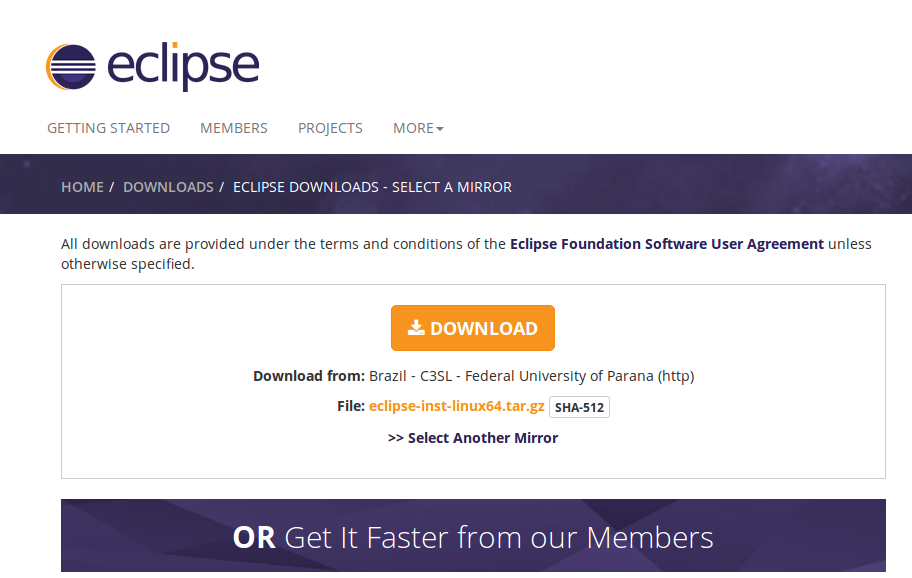
\includegraphics[height=8cm,keepaspectratio=true,clip=true]{imagenes/Apendice/eclipse1.png}
  \caption{Eclipse}
\end{figure}

Se Descarga un archivo comprimido; descomprimimos el archivo e ingresamos a la carpeta descomprimida y ejecutamos el archivo 
\textbf{eclipse.exe}. En la pantalla siguiente seleccionamos que versión de Eclipse descargar, en este caso Java Developers Eclipse.

\begin{figure}[h]
 \centering
  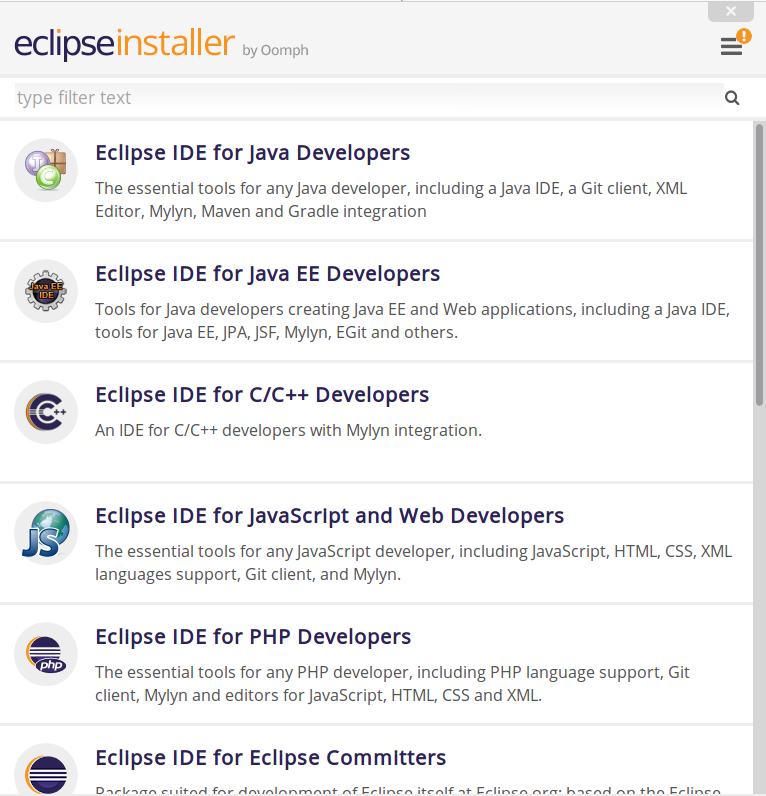
\includegraphics[height=8cm,keepaspectratio=true,clip=true]{imagenes/Apendice/eclipse2.png}
  \caption{Eclipse Instalación}
\end{figure}

\begin{figure}[h]
 \centering
  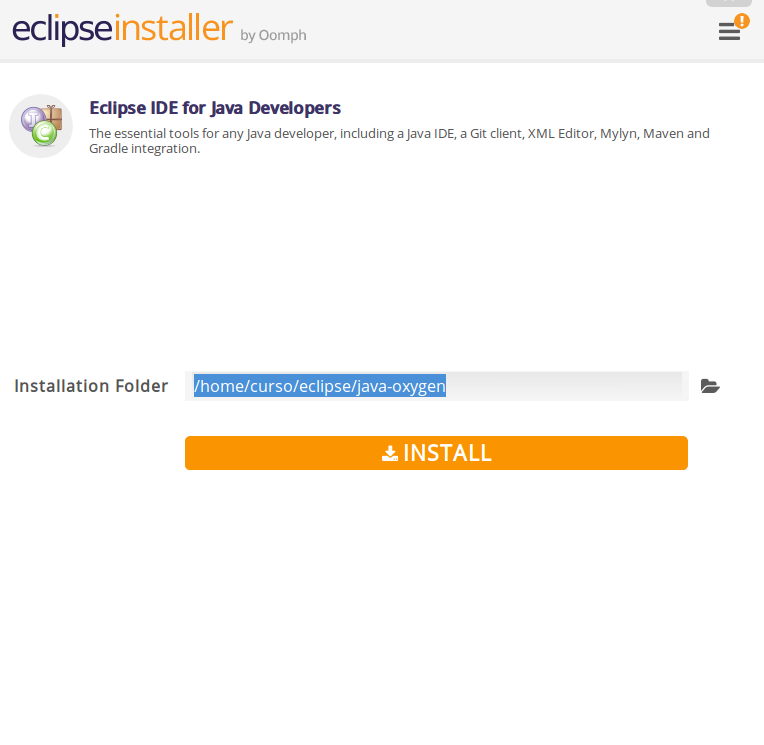
\includegraphics[height=8cm,keepaspectratio=true,clip=true]{imagenes/Apendice/eclipse3.png}
  \caption{Eclipse Instalación}
\end{figure}

\begin{figure}[h]
 \centering
  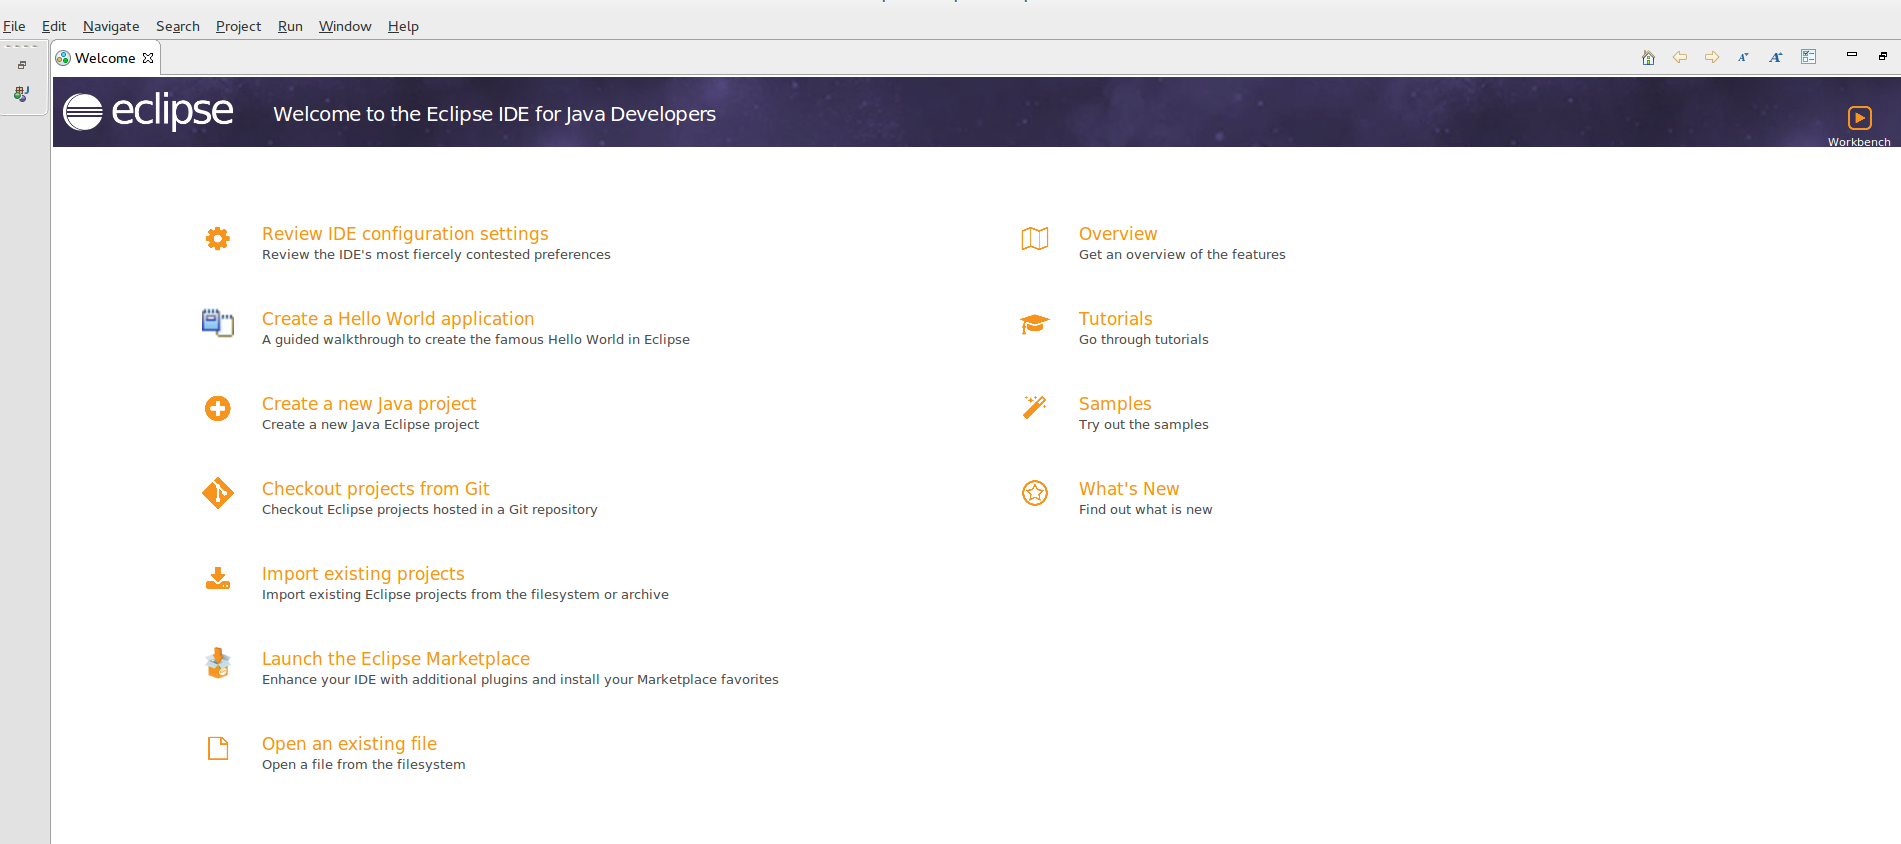
\includegraphics[height=8cm,keepaspectratio=true,clip=true]{imagenes/Apendice/eclipse4.png}
  \caption{Eclipse Entorno Principal}
\end{figure}


\subsubsection*{Plug-ins}
Para la instalación de los \textit{plug-ins} se siguió los siguientes pasos: \textit{Help->EclipseMarketplace} buscar los plug-ins \textit{Pydev} y 
\textit{Egit}. Reiniciar la herramienta para que tome las instalaciones realizadas.
\begin{figure}[h]
 \centering
  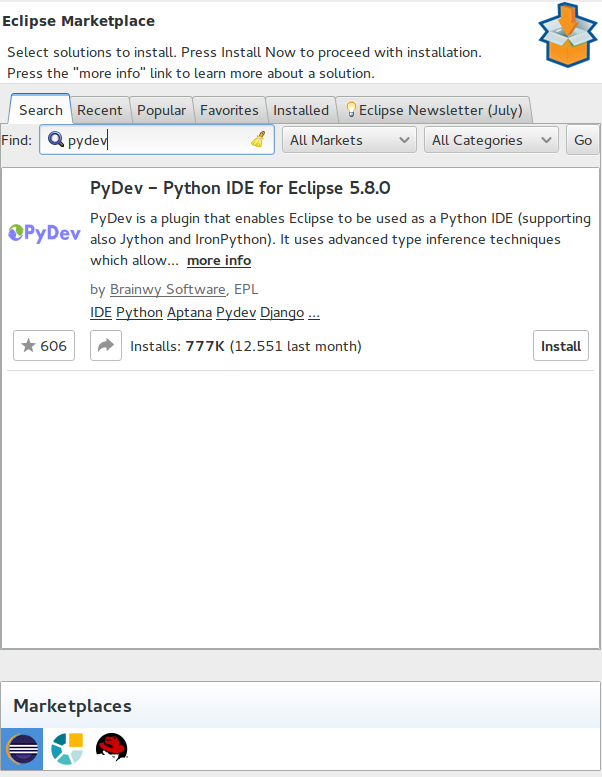
\includegraphics[height=8cm,keepaspectratio=true,clip=true]{imagenes/Apendice/eclipse5.png}
  \caption{Eclipse instalación plug-ins}
\end{figure}


